%auto-ignore
\ifx\compilefullpaper\undefined  
\documentclass[11pt]{article}
%auto-ignore
\usepackage{fullpage}
\usepackage{amsfonts, amssymb, amsmath, amsthm}
\usepackage{latexsym}
\usepackage[tracking=smallcaps]{microtype}	% for an arXiv submission, set \pdfoutput=1 near the top so it uses pdflatex
\usepackage{url}
\usepackage{color}
\definecolor{DarkGray}{rgb}{0.1,0.1,0.5}
\usepackage[colorlinks=true,breaklinks, linkcolor=black,citecolor=black,urlcolor=DarkGray]{hyperref}	% linkcolor=blue,citecolor=blue,urlcolor=blue %DarkGray

\usepackage{graphicx}
\usepackage[tight, TABBOTCAP]{subfigure}
%\usepackage{cancel}
%\usepackage{multirow}
%\usepackage[small]{caption}	%% caption package is useful for allowing line breaks within figure captions

%\usepackage{import}
%\usepackage{longtable}
%\usepackage{booktabs}
%\usepackage{ltxtable}
%\usepackage{rotating}	%% rotating package defines sideways environment

%\usepackage{calc}	%% The calc package reimplements the LaTeX commands \setcounter, ..., so that these commands accept an infix notation expression.

%\let\oldbibliography\thebibliography
%\renewcommand{\thebibliography}[1]{%
%  \oldbibliography{#1}%
%  \setlength{\itemsep}{.25pt}%
%}

%\usepackage[letterpaper]{geometry}		\geometry{includefoot,verbose,nohead,tmargin=1in,bmargin=.75in,lmargin=1.5in,rmargin=1in}
%\setlength{\parindent}{0.25in} \setlength{\parskip}{6pt}	\renewcommand{\baselinestretch}{1.66}	% stretch things out
%\def\ssp{\def\baselinestretch{1.0}\large\normalsize}	% single-space references

\def\place #1#2#3{\mspace{#2}\makebox[0pt]{\raisebox{#3}{#1}}\mspace{-#2}}	% the second argument should be in mu, and the third argument in pt

%%    Q-circuit version 2
%    Copyright (C) 2004  Steve Flammia & Bryan Eastin
%    Last modified on: 9/16/2011
%
%    This program is free software; you can redistribute it and/or modify
%    it under the terms of the GNU General Public License as published by
%    the Free Software Foundation; either version 2 of the License, or
%    (at your option) any later version.
%
%    This program is distributed in the hope that it will be useful,
%    but WITHOUT ANY WARRANTY; without even the implied warranty of
%    MERCHANTABILITY or FITNESS FOR A PARTICULAR PURPOSE.  See the
%    GNU General Public License for more details.
%
%    You should have received a copy of the GNU General Public License
%    along with this program; if not, write to the Free Software
%    Foundation, Inc., 59 Temple Place, Suite 330, Boston, MA  02111-1307  USA

% Thanks to the Xy-pic guys, Kristoffer H Rose, Ross Moore, and Daniel Müllner,
% for their help in making Qcircuit work with Xy-pic version 3.8.  
% Thanks also to Dave Clader, Andrew Childs, Rafael Possignolo, Tyson Williams,
% Sergio Boixo, Cris Moore, Jonas Anderson, and Stephan Mertens for helping us test 
% and/or develop the new version.

\usepackage{xy}
\xyoption{matrix}
\xyoption{frame}
\xyoption{arrow}
\xyoption{arc}

\usepackage{ifpdf}
\ifpdf
\else
\PackageWarningNoLine{Qcircuit}{Qcircuit is loading in Postscript mode.  The Xy-pic options ps and dvips will be loaded.  If you wish to use other Postscript drivers for Xy-pic, you must modify the code in Qcircuit.tex}
%    The following options load the drivers most commonly required to
%    get proper Postscript output from Xy-pic.  Should these fail to work,
%    try replacing the following two lines with some of the other options
%    given in the Xy-pic reference manual.
\xyoption{ps}
\xyoption{dvips}
\fi

% The following resets Xy-pic matrix alignment to the pre-3.8 default, as
% required by Qcircuit.
\entrymodifiers={!C\entrybox}

\newcommand{\bra}[1]{{\left\langle{#1}\right\vert}}
\newcommand{\ket}[1]{{\left\vert{#1}\right\rangle}}
    % Defines Dirac notation. %7/5/07 added extra braces so that the commands will work in subscripts.
\newcommand{\qw}[1][-1]{\ar @{-} [0,#1]}
    % Defines a wire that connects horizontally.  By default it connects to the object on the left of the current object.
    % WARNING: Wire commands must appear after the gate in any given entry.
\newcommand{\qwx}[1][-1]{\ar @{-} [#1,0]}
    % Defines a wire that connects vertically.  By default it connects to the object above the current object.
    % WARNING: Wire commands must appear after the gate in any given entry.
\newcommand{\cw}[1][-1]{\ar @{=} [0,#1]}
    % Defines a classical wire that connects horizontally.  By default it connects to the object on the left of the current object.
    % WARNING: Wire commands must appear after the gate in any given entry.
\newcommand{\cwx}[1][-1]{\ar @{=} [#1,0]}
    % Defines a classical wire that connects vertically.  By default it connects to the object above the current object.
    % WARNING: Wire commands must appear after the gate in any given entry.
\newcommand{\gate}[1]{*+<.6em>{#1} \POS ="i","i"+UR;"i"+UL **\dir{-};"i"+DL **\dir{-};"i"+DR **\dir{-};"i"+UR **\dir{-},"i" \qw}
    % Boxes the argument, making a gate.
\newcommand{\meter}{*=<1.8em,1.4em>{\xy ="j","j"-<.778em,.322em>;{"j"+<.778em,-.322em> \ellipse ur,_{}},"j"-<0em,.4em>;p+<.5em,.9em> **\dir{-},"j"+<2.2em,2.2em>*{},"j"-<2.2em,2.2em>*{} \endxy} \POS ="i","i"+UR;"i"+UL **\dir{-};"i"+DL **\dir{-};"i"+DR **\dir{-};"i"+UR **\dir{-},"i" \qw}
    % Inserts a measurement meter.
    % In case you're wondering, the constants .778em and .322em specify
    % one quarter of a circle with radius 1.1em.
    % The points added at + and - <2.2em,2.2em> are there to strech the
    % canvas, ensuring that the size is unaffected by erratic spacing issues
    % with the arc.
\newcommand{\measure}[1]{*+[F-:<.9em>]{#1} \qw}
    % Inserts a measurement bubble with user defined text.
\newcommand{\measuretab}[1]{*{\xy*+<.6em>{#1}="e";"e"+UL;"e"+UR **\dir{-};"e"+DR **\dir{-};"e"+DL **\dir{-};"e"+LC-<.5em,0em> **\dir{-};"e"+UL **\dir{-} \endxy} \qw}
    % Inserts a measurement tab with user defined text.
\newcommand{\measureD}[1]{*{\xy*+=<0em,.1em>{#1}="e";"e"+UR+<0em,.25em>;"e"+UL+<-.5em,.25em> **\dir{-};"e"+DL+<-.5em,-.25em> **\dir{-};"e"+DR+<0em,-.25em> **\dir{-};{"e"+UR+<0em,.25em>\ellipse^{}};"e"+C:,+(0,1)*{} \endxy} \qw}
    % Inserts a D-shaped measurement gate with user defined text.
\newcommand{\multimeasure}[2]{*+<1em,.9em>{\hphantom{#2}} \qw \POS[0,0].[#1,0];p !C *{#2},p \drop\frm<.9em>{-}}
    % Draws a multiple qubit measurement bubble starting at the current position and spanning #1 additional gates below.
    % #2 gives the label for the gate.
    % You must use an argument of the same width as #2 in \ghost for the wires to connect properly on the lower lines.
\newcommand{\multimeasureD}[2]{*+<1em,.9em>{\hphantom{#2}} \POS [0,0]="i",[0,0].[#1,0]="e",!C *{#2},"e"+UR-<.8em,0em>;"e"+UL **\dir{-};"e"+DL **\dir{-};"e"+DR+<-.8em,0em> **\dir{-};{"e"+DR+<0em,.8em>\ellipse^{}};"e"+UR+<0em,-.8em> **\dir{-};{"e"+UR-<.8em,0em>\ellipse^{}},"i" \qw}
    % Draws a multiple qubit D-shaped measurement gate starting at the current position and spanning #1 additional gates below.
    % #2 gives the label for the gate.
    % You must use an argument of the same width as #2 in \ghost for the wires to connect properly on the lower lines.
\newcommand{\control}{*!<0em,.025em>-=-<.2em>{\bullet}}
    % Inserts an unconnected control.
\newcommand{\controlo}{*+<.01em>{\xy -<.095em>*\xycircle<.19em>{} \endxy}}
    % Inserts a unconnected control-on-0.
\newcommand{\ctrl}[1]{\control \qwx[#1] \qw}
    % Inserts a control and connects it to the object #1 wires below.
\newcommand{\ctrlo}[1]{\controlo \qwx[#1] \qw}
    % Inserts a control-on-0 and connects it to the object #1 wires below.
\newcommand{\targ}{*+<.02em,.02em>{\xy ="i","i"-<.39em,0em>;"i"+<.39em,0em> **\dir{-}, "i"-<0em,.39em>;"i"+<0em,.39em> **\dir{-},"i"*\xycircle<.4em>{} \endxy} \qw}
    % Inserts a CNOT target.
\newcommand{\qswap}{*=<0em>{\times} \qw}
    % Inserts half a swap gate.
    % Must be connected to the other swap with \qwx.
\newcommand{\multigate}[2]{*+<1em,.9em>{\hphantom{#2}} \POS [0,0]="i",[0,0].[#1,0]="e",!C *{#2},"e"+UR;"e"+UL **\dir{-};"e"+DL **\dir{-};"e"+DR **\dir{-};"e"+UR **\dir{-},"i" \qw}
    % Draws a multiple qubit gate starting at the current position and spanning #1 additional gates below.
    % #2 gives the label for the gate.
    % You must use an argument of the same width as #2 in \ghost for the wires to connect properly on the lower lines.
\newcommand{\ghost}[1]{*+<1em,.9em>{\hphantom{#1}} \qw}
    % Leaves space for \multigate on wires other than the one on which \multigate appears.  Without this command wires will cross your gate.
    % #1 should match the second argument in the corresponding \multigate.
\newcommand{\push}[1]{*{#1}}
    % Inserts #1, overriding the default that causes entries to have zero size.  This command takes the place of a gate.
    % Like a gate, it must precede any wire commands.
    % \push is useful for forcing columns apart.
    % NOTE: It might be useful to know that a gate is about 1.3 times the height of its contents.  I.e. \gate{M} is 1.3em tall.
    % WARNING: \push must appear before any wire commands and may not appear in an entry with a gate or label.
\newcommand{\gategroup}[6]{\POS"#1,#2"."#3,#2"."#1,#4"."#3,#4"!C*+<#5>\frm{#6}}
    % Constructs a box or bracket enclosing the square block spanning rows #1-#3 and columns=#2-#4.
    % The block is given a margin #5/2, so #5 should be a valid length.
    % #6 can take the following arguments -- or . or _\} or ^\} or \{ or \} or _) or ^) or ( or ) where the first two options yield dashed and
    % dotted boxes respectively, and the last eight options yield bottom, top, left, and right braces of the curly or normal variety.  See the Xy-pic reference manual for more options.
    % \gategroup can appear at the end of any gate entry, but it's good form to pick either the last entry or one of the corner gates.
    % BUG: \gategroup uses the four corner gates to determine the size of the bounding box.  Other gates may stick out of that box.  See \prop.

\newcommand{\rstick}[1]{*!L!<-.5em,0em>=<0em>{#1}}
    % Centers the left side of #1 in the cell.  Intended for lining up wire labels.  Note that non-gates have default size zero.
\newcommand{\lstick}[1]{*!R!<.5em,0em>=<0em>{#1}}
    % Centers the right side of #1 in the cell.  Intended for lining up wire labels.  Note that non-gates have default size zero.
\newcommand{\ustick}[1]{*!D!<0em,-.5em>=<0em>{#1}}
    % Centers the bottom of #1 in the cell.  Intended for lining up wire labels.  Note that non-gates have default size zero.
\newcommand{\dstick}[1]{*!U!<0em,.5em>=<0em>{#1}}
    % Centers the top of #1 in the cell.  Intended for lining up wire labels.  Note that non-gates have default size zero.
\newcommand{\Qcircuit}{\xymatrix @*=<0em>}
    % Defines \Qcircuit as an \xymatrix with entries of default size 0em.
\newcommand{\link}[2]{\ar @{-} [#1,#2]}
    % Draws a wire or connecting line to the element #1 rows down and #2 columns forward.
\newcommand{\pureghost}[1]{*+<1em,.9em>{\hphantom{#1}}}
    % Same as \ghost except it omits the wire leading to the left. 

%\renewcommand{\measureD}[1]{*{\xy*+=+<.5em>{\vphantom{\rule{0em}{.1em}#1}}*\cir{r_l};p\save*!R{#1} \restore\save+UC;+UC-<.15em,0em>*!R{\hphantom{#1}}+L **\dir{-} \restore\save+DC;+DC-<.15em,0em>*!R{\hphantom{#1}}+L **\dir{-} \restore\POS+UC-<.1em,0em>*!R{\hphantom{#1}}+L;+DC-<.15em,0em>*!R{\hphantom{#1}}+L **\dir{-} \endxy} \qw}
\newcommand{\redcontrol}{*!<0em,.025em>-=-{\color{red}\bullet\color{black}}}
\newcommand{\redqwx}[1][-1]{\color{red}\ar @{-} [#1,0]\color{black}}
\newcommand{\redctrl}[1]{\redcontrol \redqwx[#1] \qw}
\newcommand{\redtarg}{*!<0em,.019em>=<.79em,.68em>{\color{red}\xy {<0em,0em>*{} \ar @{ - } +<.4em,0em> \ar @{ - } -<.4em,0em> \ar @{ - } +<0em,.36em> \ar @{ - } -<0em,.36em>},<0em,-.019em>*+<.8em>\frm{o}\endxy} \color{black}\qw}

\newcommand{\bra}[1]{{\langle#1|}}
\newcommand{\ket}[1]{{|#1\rangle}}
\newcommand{\braket}[2]{{\langle#1|#2\rangle}}
\newcommand{\ketbra}[2]{{\ket{#1}\!\bra{#2}}}
\newcommand{\lbra}[1]{{\bra{\overline{#1}}}}
\newcommand{\lket}[1]{{\ket{\overline{#1}}}}
\newcommand{\abs}[1]{{\lvert #1\rvert}}	% since the delimiters do not scale, it might be a good idea to add a dummy {} at the end, so \abs{big expression}^2 has the superscript at a low height
\newcommand{\bigabs}[1]{{\big\lvert #1\big\rvert}}
\newcommand{\Bigabs}[1]{{\Big\lvert #1\Big\rvert}}

\newcommand{\norm}[1]{{\| #1 \|}}
\newcommand{\bignorm}[1]{{\big\| #1 \big\|}}
\newcommand{\Bignorm}[1]{{\Big\| #1 \Big\|}}
\newcommand{\Biggnorm}[1]{{\Bigg\| #1 \Bigg\|}}
%\newcommand{\trnorm}[1]{{\norm{#1}_{\mathrm{tr}}}}
\newcommand{\trnorm}[1]{{\| #1 \|_{\mathrm{tr}}}}
\newcommand{\bigtrnorm}[1]{{\bigl\| #1 \bigr\|_{\mathrm{tr}}}}	% by not calling \bignorm, the subscript height is independent of the argument
\newcommand{\Bigtrnorm}[1]{{\Bigl\| #1 \Bigr\|_{\mathrm{tr}}}}
\newcommand{\Biggtrnorm}[1]{{\Biggl\| #1 \Biggr\|_{\mathrm{tr}}}}

\newcommand{\eps}{{\epsilon}}
\newcommand{\binomial}[2]{\ensuremath{\left(\begin{smallmatrix}#1 \\ #2 \end{smallmatrix}\right)}}
\newcommand{\fastmatrix}[1]{\left(\begin{smallmatrix}#1\end{smallmatrix}\right)}
\newcommand{\smatrx}[1]{\ensuremath{\left(\begin{smallmatrix}#1\end{smallmatrix}\right)}}
\newcommand{\matrx}[1]{\ensuremath{\left(\begin{matrix}#1\end{matrix}\right)}}
\DeclareMathOperator{\Ex}{\operatorname{E}}
\DeclareMathOperator{\Tr}{\operatorname{Tr}}

\def\tensor {\otimes}
\def\adjoint{\dagger} %{*}

\def\A {{\mathcal A}}
\def\B {{\mathcal B}}
\def\C {{\bf C}}
\def\D {{\mathcal D}}
\def\E {{\mathcal E}}
\def\F {{\mathcal F}}
\def\G {{\mathcal G}}
\def\H {{\mathcal H}}
\let\Lstroke\L	\def\L {{\mathcal L}}		
\def\N {{\bf N}}
\def\cP {{\mathcal P}}
\def\R {{\bf R}}
\def\S {{\mathcal S}}
\def\U {{\mathcal U}}
\def\V {{\mathcal V}}

%% Complexity classes: 
\renewcommand{\P}{\ensuremath{\mathsf{P}}}%{{\mathcal{NP}}}
\newcommand{\NP}{\ensuremath{\mathsf{NP}}}%{{\mathcal{NP}}}
\newcommand{\IP}{\ensuremath{\mathsf{IP}}}%{{\mathcal{NP}}}
\newcommand{\PSPACE}{\ensuremath{\mathsf{PSPACE}}}%{{\mathcal{NP}}}
\newcommand{\BQP}{\ensuremath{\mathsf{BQP}}}%{{\mathcal{BQP}}}
\newcommand{\EXP}{\ensuremath{\mathsf{EXP}}}%{{\mathcal{NP}}}
\newcommand{\NEXP}{\ensuremath{\mathsf{NEXP}}}%{{\mathcal{NP}}}
\newcommand{\QIP}{\ensuremath{\mathsf{QIP}}}%{{\mathcal{NP}}}
\newcommand{\QMIP}{\ensuremath{\mathsf{QMIP}}}%{{\mathcal{NP}}}
\newcommand{\MIP}{\ensuremath{\mathsf{MIP}}}%{{\mathcal{NP}}}

\DeclareMathOperator{\Span}{\operatorname{Span}}
\DeclareMathOperator{\Range}{\operatorname{Range}}
\DeclareMathOperator{\Kernel}{\operatorname{Ker}}
\DeclareMathOperator{\poly}{\operatorname{poly}}
\DeclareMathOperator{\qpoly}{\operatorname{qpoly}}
\DeclareMathOperator{\rank}{\operatorname{rank}}
\newcommand{\identity}{\ensuremath{\boldsymbol{1}}} %\mathbb{I}
\newcommand{\Id}{\identity} 
\DeclareMathOperator{\CNOT}{\operatorname{CNOT}}
\DeclareMathOperator{\SWAP}{\operatorname{SWAP}}

%\newtheorem*{maintheorem}{Main Theorem}

\newcommand{\hugelpar}[1]{\left(\vbox to #1{}\right.}
\newcommand{\hugerpar}[1]{\left.\vbox to #1{}\right)}
\newcounter{sprows}
\newcounter{spcols}
\newlength{\spheight}
\newlength{\spraise}
\newcommand{\spleft}[2][0pt]{\multirow{\value{sprows}}{*}{%
	\vbox to \spraise{\vss\hbox{$#2 \hugelpar{\spheight}\hskip -#1$}\vss}}}
\newcommand{\spright}[2][0pt]{\multirow{\value{sprows}}{*}{%
	\vbox to \spraise{\vss\hbox{\hskip -#1 $\hugerpar{\spheight} #2$}\vss}}}

\newcommand{\comment}[1]{\emph{\color{blue}Comment:\color{black} #1}} % use for simply removing comments
\newlength{\commentslength}
\newcommand{\comments}[1]{
\hspace{-2\parindent}
\addtolength{\commentslength}{-\commentslength}
\addtolength{\commentslength}{\linewidth}
\addtolength{\commentslength}{-\parindent}
\fcolorbox{blue}{white}{\smallskip\begin{minipage}[c]{\commentslength}
\emph{Comments:}\begin{itemize}#1\end{itemize}\end{minipage}}\bigskip
}
%\renewcommand{\comment}[1]{}\renewcommand{\comments}[1]{}
\newcommand{\rem}[1]{}

%\numberwithin{equation}{section} % makes Eq. numbers (section.number)

\newtheorem{theorem}{Theorem}[section]
\newtheorem{lemma}[theorem]{Lemma}
\newtheorem{corollary}[theorem]{Corollary}
\newtheorem{claim}[theorem]{Claim}
\newtheorem{fact}[theorem]{Fact}
\newtheorem{proposition}[theorem]{Proposition}
\newtheorem{conjecture}[theorem]{Conjecture}

%\theoremstyle{definition}
\newtheorem{definition}[theorem]{Definition}
\newtheorem{condition}[theorem]{Condition}
%\theoremstyle{remark}
\newtheorem{remark}[theorem]{Remark}
%% some font options include \itshape (preferred), \slshape (same as italic, but with broader spacing), \bfseries (bold), \normalfont
%\newtheoremstyle{definition}{}{}{\normalfont}{}{\itshape}{.}{ }{}
%\theoremstyle{definition}
\newtheorem{example}[theorem]{Example}

\newfont{\subsubsecfnt}{ptmri8t at 11pt}
\renewcommand{\subparagraph}[1]{\smallskip{\subsubsecfnt #1.}}

%% The first versions below hyperlink the whole reference, while the second versions only hyperlink the number
\newcommand{\eqnref}[1]{\hyperref[#1]{{(\ref*{#1})}}}
\newcommand{\thmref}[1]{\hyperref[#1]{{Theorem~\ref*{#1}}}}
\newcommand{\lemref}[1]{\hyperref[#1]{{Lemma~\ref*{#1}}}}
\newcommand{\corref}[1]{\hyperref[#1]{{Corollary~\ref*{#1}}}}
\newcommand{\defref}[1]{\hyperref[#1]{{Definition~\ref*{#1}}}}
\newcommand{\secref}[1]{\hyperref[#1]{{Section~\ref*{#1}}}}
\newcommand{\figref}[1]{\hyperref[#1]{{Figure~\ref*{#1}}}}
\newcommand{\tabref}[1]{\hyperref[#1]{{Table~\ref*{#1}}}}
\newcommand{\remref}[1]{\hyperref[#1]{{Remark~\ref*{#1}}}}
\newcommand{\appref}[1]{\hyperref[#1]{{Appendix~\ref*{#1}}}}
\newcommand{\claimref}[1]{\hyperref[#1]{{Claim~\ref*{#1}}}}
\newcommand{\factref}[1]{\hyperref[#1]{{Fact~\ref*{#1}}}}
\newcommand{\propref}[1]{\hyperref[#1]{{Proposition~\ref*{#1}}}}
\newcommand{\exampleref}[1]{\hyperref[#1]{{Example~\ref*{#1}}}}
\newcommand{\conjref}[1]{\hyperref[#1]{{Conjecture~\ref*{#1}}}}

%
%\newcommand{\eqnref}[1]{{(\hyperref[#1]{\ref*{#1}})}}
%\newcommand{\thmref}[1]{{Theorem~\hyperref[#1]{\ref*{#1}}}}
%\newcommand{\lemref}[1]{{Lemma~\hyperref[#1]{\ref*{#1}}}}
%\newcommand{\corref}[1]{{Corollary~\hyperref[#1]{\ref*{#1}}}}
%\newcommand{\defref}[1]{{Definition~\hyperref[#1]{\ref*{#1}}}}
%\newcommand{\secref}[1]{{Section~\hyperref[#1]{\ref*{#1}}}}
%\newcommand{\figref}[1]{{Figure~\hyperref[#1]{\ref*{#1}}}}
%\newcommand{\tabref}[1]{{Table~\hyperref[#1]{\ref*{#1}}}}
%\newcommand{\remref}[1]{{Remark~\hyperref[#1]{\ref*{#1}}}}
%\newcommand{\appref}[1]{{Appendix~\hyperref[#1]{\ref*{#1}}}}
%\newcommand{\claimref}[1]{{Claim~\hyperref[#1]{\ref*{#1}}}}
%\newcommand{\propref}[1]{{Proposition~\hyperref[#1]{\ref*{#1}}}}
%\newcommand{\exampleref}[1]{{Example~\hyperref[#1]{\ref*{#1}}}}
%\newcommand{\conjref}[1]{{Conjecture~\hyperref[#1]{\ref*{#1}}}}

\allowdisplaybreaks[1]
%\sloppy

%% Paper-specific macros:
\newcommand{\ADV} {\mathrm{Adv}}
\newcommand{\ADVpm} {\mathrm{Adv}^{\pm}}
\def\CZ {C\!Z}	% control-Z gate
\DeclareMathOperator{\abst}{\operatorname{abs}}
%\newcommand{\B}{B}	% \{0,1\}	{{\bf Z}_2}

\DeclareMathOperator{\depth}{\operatorname{depth}}
\DeclareMathOperator{\AND}{\ensuremath{\operatorname{AND}}}
\DeclareMathOperator{\OR}{\ensuremath{\operatorname{OR}}}
\DeclareMathOperator{\MAJ}{{\operatorname{MAJ}_3}}
\DeclareMathOperator{\EQUAL}{{\operatorname{EQUAL}}}
\DeclareMathOperator{\EXACT}{{\operatorname{EXACT}}}

\def\COLOR{}
\ifdefined\COLOR
\newcommand{\Alice}[1] {{\color{red} {#1}}}
\newcommand{\Bob}[1] {{\color{blue} {#1}}}
\else
\newcommand{\Alice}[1] {{\color{black} {#1}}}
\newcommand{\Bob}[1] {{\color{black} {#1}}}
\fi

\newcommand{\EPRstate}{{\mathrm{EPR}}}

\DeclareMathOperator{\ima}{Im}

\usepackage{array}
\begin{document}
%\tableofcontents
\fi


\section{State-dependent qubit separation} \label{s:statedependent}

A problem with both \thmref{t:manynearlyindependentqubits} and \thmref{t:swappingmanynearlyindependentqubits} is that they might be difficult to apply to real experimental systems.  This is because it is difficult to establish the assumption of qubits nearly in tensor product, $\norm{[S_i, T_j]} \leq \epsilon$ for $i \neq j$ and $S, T\in\{X,Z\}$.  In addition to the operators, a physical system involves an underlying state~$\ket \psi$.  The operators can be understood only in terms of their effects on $\ket \psi$.  Consider for example a Hilbert space that splits as $\H \oplus \H'$, where $\ket \psi$ is supported only on $\H$ and available operators leave $\H$ invariant.  Then there is no experimental way to fathom the operators' behavior, e.g., their commutation relationships, on~$\H'$.  Theorems~\ref{t:manynearlyindependentqubits} and~\ref{t:swappingmanynearlyindependentqubits} cannot be applied.  This example might not seem so troubling, because we can simply restrict everything to~$\H$; but it becomes more problematic if $\ket \psi$, say, has nonzero but very small support on~$\H'$.  

We would like qubit-separation theorems that have experimentally accessible assumptions.  In particular, the theorems' assumptions should be stated relative to the system's state~$\ket \psi$.  For example, in Theorems~\ref{t:manynearlyindependentqubits} and~\ref{t:swappingmanynearlyindependentqubits} we might loosen the assumption $\norm{[S_i, T_j]} \leq \epsilon$ for $i \neq j$ to be only $\norm{[S_i, T_j] \ket \psi} \leq \epsilon$.  Naturally, the conclusions will have to be correspondingly weakened.  In the above example with $\H \oplus \H'$, if the reflections are far from commuting on~$\H'$ then we cannot hope to find nearby commuting operators, $\norm{S_j' - S_j} \approx 0$; but perhaps we can get $\norm{(S_j' - S_j) \ket \psi} \approx 0$.  

In order to extend our results to experimental systems we proceed in three steps.  

\begin{enumerate}
\item 
First, in \secref{s:statedependentcommutationprotocol} below, we give a protocol that can be used to test if two reflections, $S$ and~$T$, are close to commuting on a state~$\ket \psi$: $[S, T] \ket \psi \approx 0$.  The protocol is very simple: measure $S$, measure $T$, then measure $S$ again.  If $S$ and~$T$ commute on~$\ket \psi$, then the two $S$ measurements will give the same result; and, intuitively, when they do not commute measuring $T$ will disturb the state and make it less likely to get the same $S$ result.  

\item 
However, in \secref{s:statedependentseparationcounterexample}, we show that the condition $[S_i, T_j] \ket \psi \approx 0$ for operators on different qubits is not sufficient to establish that there are nearby independent qubits $X_1', Z_1', \ldots, X_n', Z_n'$.  In fact, we give an explicit construction of a state~$\ket \psi$ and $n$ qubit operators $X_1, Z_1, \ldots, X_n, Z_n$ in $< n^2$ dimensions such that for $i \neq j$, $[S_i, T_j] \ket \psi = 0$ precisely.  Since $n^2 \leq 2^n$ for $n \geq 4$, the dimension of the space is not sufficient to fit $n$ independent qubits.  

(We also show why the basic induction argument used to prove \thmref{t:manynearlyindependentqubits} fails when errors are measured relative to a state~$\ket \psi$.  The errors accumulate too rapidly, leading to an exponential dependence on~$n$, instead of polynomial.)  

\item 
We remedy this problem in \secref{s:statedependentnqubitprotocol} with a more advanced testing protocol.  Intuitively, the improved protocol tests not just pairwise commutation relationships, such as $S_i T_j \ket \psi \approx T_j S_i \ket \psi$, but also higher-order relationships such as $S_i T_j U_k \ket \psi \approx U_k T_j S_i \ket \psi$.  The protocol is still quite simple, though.  Basically, measure all the qubit operators in order (either $X_1, Z_1, X_2, Z_2, \ldots$ or $Z_1, X_1, Z_2, X_2, \ldots$), then go back and measure a random qubit operator ($Z_j$ or $X_j$, respectively), and verify that the measurement result is unchanged.  We show that if the protocol accepts with probability $1 - \epsilon$, then the qubit operators ``simulate'' $n$ independent qubit operators in a certain sense.  In particular, as a corollary, the system's dimension must be at least $(1 - O(n^2 \epsilon)) 2^n$.  

The dimension bound is not fully satisfactory.  A $2^n$ lower bound would be preferable.  However, speculatively, the simulation statement might be strong enough to form the foundation for an analysis that the system can be used as an $n$-qubit quantum computer.  Such an extension is nontrivial, though, and we leave it to future work.  
\end{enumerate}


\medskip %
\subsection{Protocol for testing state-dependent commutation} \label{s:statedependentcommutationprotocol}

We present a protocol that can be used to test whether two reflections approximately commute on a given state.  

\medskip %

\begin{theorem} \label{t:statedependentcommutationprotocol}
Let $S$ and~$T$ be reflections, acting on a state~$\ket \psi$.  Consider the following protocol: 
\begin{enumerate}
\item Measure $S$.  
\item Measure $T$, but ignore the result.    
\item Measure $S$ again.  Accept if the result is unchanged.  
\end{enumerate}
Then the probability of accepting is given by 
\begin{equation*}
\Pr[\mathrm{accept}] = 1 - \tfrac18 \bignorm{[S, T] \ket \psi}{}^2
 \enspace .
\end{equation*}
\end{theorem}


\begin{proof}
For $a, b \in \{0, 1\}$, let $S_a = \tfrac12 (\Id + (-1)^a S)$ and $T_b = \tfrac12 (\Id + (-1)^b T)$.  Then since $[S, T_0] = -[S, T_1] = \tfrac12 [S, T]$, 
\begin{align*}
\norm{[S, T] \ket \Psi}^2
&= 2 \big( \norm{ [S, T_0] \ket \psi }^2 + \norm{ [S, T_1] \ket \psi }^2 \big) \\
&= \sum_{a, b} \bignorm{S_a [S, T_b] \ket \psi}^2 
 \enspace , 
\intertext{where we have used $\norm{\ket \phi}^2 = \norm{S_0 \ket \phi}^2 + \norm{S_1\ket \phi}^2$ for any $\ket \phi$.  Then from $S_a S = S S_a = (-1)^a S_a$, we find $S_a [S, T_b] = S_a [S, T_b] (S_0 + S_1) = 2 (-1)^a S_a T S_{\bar a}$, so }
\norm{[S, T] \ket \psi}^2
&= 8 \sum_{a, b} \bignorm{S_a T_b S_{\bar a} \ket \psi}^2 \\
&= 8 \, (1 - \Pr[\mathrm{accept}])
 \enspace .  \qedhere
\end{align*}
\end{proof}


\subsection{Qubits that commute on a state need not be close to independent qubits}
\label{s:statedependentseparationcounterexample}

In the projection separating argument of \thmref{t:manynearlycommutingprojections}, the key observation was that for projections $P$, $Q$, $R$ with $\norm{[P,Q]}, \norm{[P,R]} \leq \delta$ and $\norm{[Q,R]} \leq \epsilon$, if $Q$ and $R$ are both block-diagonalized with respect to~$P$ then the results still nearly commute:  
\begin{equation*}
\left\Vert \big[ PQP + (\identity-P)Q(\identity-P), PRP + (\identity-P)R(\identity-P) \big] \right\Vert \leq \epsilon + 2 \delta^2
 \enspace .
\end{equation*}
The quadratic dependence on $\delta$ meant that errors did not accumulate badly through the induction.  

Here is a counterexample showing that errors \emph{can} accumulate badly in block diagonalization if we measure errors relative to a state $\ket \psi$, using $\norm{[P,Q] \ket \psi}$.  Define $P$, $Q$, $R$ and $\ket \psi$ as 
\begin{equation}
P = \fastmatrix{
1 & 0 & 0 & \delta \\
0 & 1/2 & 1/2 & 0 \\
0 & 1/2 & 1/2 & 0 \\
\delta & 0 & 0 & 0
}
\qquad
Q = \fastmatrix{
1&0&0&0\\
0&0&0&0\\
0&0&1&0\\
0&0&0&0
}
\qquad
R = \fastmatrix{
1&0&0&0\\
0&0&0&0\\
0&0&1/2&1/2\\
0&0&1/2&1/2
}
\qquad 
\ket \psi = \fastmatrix{1\\0\\0\\0}
 \enspace .
\end{equation}
Then $P$, $Q$ and $R$ are projections (up to second order in $\delta$ for~$P$), with $\norm{[P,Q] \ket \psi}, \norm{[P,R] \ket \psi} = O(\delta)$, $[Q,R] \ket \psi = 0$, and yet 
\begin{equation*}
\left\Vert \big[ PQP + (\identity-P)Q(\identity-P), PRP + (\identity-P)R(\identity-P) \big] \ket \psi \right\Vert = \Omega(\delta)
 \enspace .
\end{equation*}
The idea is that $Q$ and $R$ commute on the first two dimensions, and are far from commuting on the last two dimensions; but this property is broken by the block diagonalization.  

This example suggests that in a simple induction argument, starting with projections $P_1, \ldots, P_n$ having pairwise commutators $\norm{[P_i, P_j] \ket \psi} \sim \epsilon$, after block-diagonalizing with respect to $P_1$, the errors can grow to $\sim 2 \epsilon$, then to $\sim 4 \epsilon$ after block-diagonalizing with respect to the new $P_2$, and so on; the errors potentially grow exponentially.  

In fact, it is not only our \emph{proof} of Theorems~\ref{t:manynearlycommutingprojections} and~\ref{t:manynearlyindependentqubits} that fails when errors are measured relative to a state~$\ket \psi$.  The theorems themselves fail, as shown by the following construction. 

\begin{lemma} \label{t:kcommute}
For any $n$ and $k \in [n]$, there exists a space $\H$ of dimension at most $1 + \sum_{j=0}^k {n \choose j}$, a vector $\ket \psi \in \H$ and $n$ qubits $X_j, Z_j$ such that 
\begin{equation*}
S^{(1)}_{j_1} \cdots S^{(k)}_{j_k} \ket \psi = S_{j_{\sigma(1)}}^{\sigma(1)} \cdots S_{j_{\sigma(k)}}^{\sigma(k)} \ket \psi
\end{equation*}
for all distinct indices $j_1, \ldots, j_k \in [n]$, $S^{(1)}, \ldots, S^{(k)} \in \{X, Z\}$, and permutations $\sigma$ of $[k]$.  
\end{lemma}

In particular, for $k = 2$, the lemma places $n$ qubits in $O(n^2)$ dimensions---for example, four qubits in~$12$ dimensions---such that $[S_i, T_j] \ket \psi = 0$ for all $i \neq j$ and $S,T\in\{X,Z\}$.    

\begin{proof}
Let us begin by explaining the $n = 4$, $k = 2$ special case of the construction.  Define $\H$ to have orthonormal basis $\ket{0000}, \ket{1000}, \ldots, \ket{0001}, \ket{1100}, \ldots, \ket{0011}, \ket d$, i.e., all $n$-bit strings of Hamming weight at most~$k$, together with an additional vector~$\ket d$.  Let~$\ket \psi = \ket{0000}$, and consider the following operators for the first qubit:
\vspace{.4cm}
\begin{gather*}
X_1 = \hspace{.5cm}
\left(
\makebox(95,43){\hspace{-.7cm}\raisebox{-1in}{$
\begin{smallmatrix}
&\rotatebox{85}{\tiny 0000}&
\rotatebox{85}{\tiny 1000}&
\rotatebox{85}{\tiny 0100}&
\rotatebox{85}{\tiny 0010}&
\rotatebox{85}{\tiny 0001}&
\rotatebox{85}{\tiny 1100}&
\rotatebox{85}{\tiny 1010}&
\rotatebox{85}{\tiny 1001}&
\rotatebox{85}{\tiny 0110}&
\rotatebox{85}{\tiny 0101}&
\rotatebox{85}{\tiny 0011}&
\rotatebox{85}{\tiny $d$} \\
\rotatebox{0}{\tiny 0000\;\;\;}&0&1& & & & & & & & & &  \\
\rotatebox{0}{\tiny 1000\;\;\;}&1&0& & & & & & & & & &  \\
\rotatebox{0}{\tiny 0100\;\;\;}& & &0& & &1& & & & & &  \\
\rotatebox{0}{\tiny 0010\;\;\;}& & & &0& & &1& & & & &  \\
\rotatebox{0}{\tiny 0001\;\;\;}& & & & &0& & &1& & & &  \\
\rotatebox{0}{\tiny 1100\;\;\;}& & &1& & &0& & & & & &  \\
\rotatebox{0}{\tiny 1010\;\;\;}& & & &1& & &0& & & & &  \\
\rotatebox{0}{\tiny 1001\;\;\;}& & & & &1& & &0& & & &  \\
\rotatebox{0}{\tiny 0110\;\;\;}& & & & & & & & &0&1& &  \\
\rotatebox{0}{\tiny 0101\;\;\;}& & & & & & & & &1&0& &  \\
\rotatebox{0}{\tiny 0011\;\;\;}& & & & & & & & & & &0&1 \\
\rotatebox{0}{\tiny $d$}& & & & & & & & & & &1&0 
\end{smallmatrix}
$}}
\right)
\place{\Huge 0}{-45mu}{10pt}
\place{\Huge 0}{-110mu}{-35pt}
\qquad\qquad
\def\minusone{\hspace{-.4cm}\text{--}1\hspace{-.2cm}}
Z_1 = \hspace{.5cm}
\left(
\makebox(95,43){\hspace{-.7cm}\raisebox{-1in}{$
\begin{smallmatrix}
&\rotatebox{85}{\tiny 0000}&
\rotatebox{85}{\tiny 1000}&
\rotatebox{85}{\tiny 0100}&
\rotatebox{85}{\tiny 0010}&
\rotatebox{85}{\tiny 0001}&
\rotatebox{85}{\tiny 1100}&
\rotatebox{85}{\tiny 1010}&
\rotatebox{85}{\tiny 1001}&
\rotatebox{85}{\tiny 0110}&
\rotatebox{85}{\tiny 0101}&
\rotatebox{85}{\tiny 0011}&
\rotatebox{85}{\tiny $d$} \\
\rotatebox{0}{\tiny 0000\;\;\;}&1& & & & & & & & & & &  \\
\rotatebox{0}{\tiny 1000\;\;\;}& &\minusone& & & & & & & & & &  \\
\rotatebox{0}{\tiny 0100\;\;\;}& & &1& & & & & & & & &  \\
\rotatebox{0}{\tiny 0010\;\;\;}& & & &1& & & & & & & &  \\
\rotatebox{0}{\tiny 0001\;\;\;}& & & & &1& & & & & & &  \\
\rotatebox{0}{\tiny 1100\;\;\;}& & & & & &\minusone& & & & & &  \\
\rotatebox{0}{\tiny 1010\;\;\;}& & & & & & &\minusone& & & & &  \\
\rotatebox{0}{\tiny 1001\;\;\;}& & & & & & & &\minusone& & & &  \\
\rotatebox{0}{\tiny 0110\;\;\;}& & & & & & & & &1& & &  \\
\rotatebox{0}{\tiny 0101\;\;\;}& & & & & & & & & &\minusone& &  \\
\rotatebox{0}{\tiny 0011\;\;\;}& & & & & & & & & & &1&  \\
\rotatebox{0}{\tiny $d$}& & & & & & & & & & & &\minusone 
\end{smallmatrix}
$}}
\right)
\place{\Huge 0}{-55mu}{10pt}
\place{\Huge 0}{-130mu}{-25pt}
 \enspace .
\end{gather*}
Unspecified matrix entries are $0$.  $X_2$ and $Z_2$ can be obtained from $X_1$ and $Z_1$ by switching the first and second bits in each basis element, leaving $\ket d$ alone; and similarly for $X_3, Z_3$ and $X_4, Z_4$.  Then $P_i^2 = \identity$, $\{X_i, Z_i\} = 0$ and $[P_i, Q_j] \ket \psi = 0$, for $i \neq j$ and $P, Q \in \{X, Z\}$.  

The idea behind this construction is that $X_j, Z_j$ act largely as the Pauli operators $\sigma^x_j, \sigma^z_j$.  However, we have truncated the standard basis $\ket{0000}, \ldots, \ket{1111}$ for $(\C^2)^{\otimes 4}$ to include only strings of Hamming weight $\leq 2$.  Since applying $\sigma^x_1$ to $\ket{0110}, \ket{0101}$ and $\ket{0011}$ would give strings of Hamming weight~$3$, we instead pair these dimensions up arbitrarily for~$X_1$, and define $Z_1$ on them to make it anti-commute with $X_1$.  The extra dimension $\ket d$ is needed to make the total dimension even.  

It is straightforward to generalize the example: by truncating strings at Hamming weight~$k$ the same construction places $n$ qubits in $\sum_{j=0}^k \big(\begin{smallmatrix}n\\j\end{smallmatrix}\big)$ dimensions (or one more if this dimension is odd), such that any combination of up to $k$ qubit operators commute on $\ket \psi = \ket{0^n}$, e.g., if $k \geq 3$, $X_1 X_2 X_3 \ket \psi = X_3 X_2 X_1 \ket \psi = \ket{1110^{n-3}}$.  
\end{proof}


\subsection{Protocol to test for $n$ independent qubits} \label{s:statedependentnqubitprotocol}

The problem with the protocol in \thmref{t:statedependentcommutationprotocol} is that it only tests commutation between pairs of operators on the state $\ket \psi$: $[S, T] \ket \psi \approx 0$.  \lemref{t:kcommute} shows that $n$ qubits in only $O(n^2)$ dimensions can pass this test on every pair.  The lemma furthermore suggests that any test involving qubit operator sequences of length $o(n)$ can be satisfied in dimension $2^{o(n)}$.  Therefore, we need a protocol that has at least~$n$ steps.  

\figref{f:statedependentnqubitprotocol} gives our testing protocol.  We argue that if the protocol accepts with high probability, then the $n$ overlapping qubits $X_j, Z_j$ are nearly equivalent to $n$ independent qubits $\hat X_j, \hat Z_j$ in an enlarged space $\H' = \H \otimes (\C^2)^{\otimes 2 n}$.  

\begin{figure}
{ \noindent \hrulefill \\
\centering \textbf{Protocol to test for $n$ independent qubits} \\ } \smallskip

Let $\ket \psi \in \H$ be a state.  Let $X_1, Z_1, \ldots, X_n, Z_n$ be qubit operators on~$\H$, i.e., reflections satisfying $\{X_j, Z_j\} = 0$ for all~$j$.  
\begin{enumerate}
\item With equal probabilities $1/2$, measure the reflections in order, either $X_1, Z_1, X_2, Z_2, \ldots$, or $Z_1, X_1, Z_2, X_2, \ldots$.  
\item Pick a uniformly random index $j \in [n]$.  If $Z$ went second in step $(1)$, then measure~$Z_j$; and if $X$ went second, then measure $X_j$.  Accept if the result is unchanged from the operator's previous measurement.  Otherwise reject.  
\end{enumerate}
\vspace{-1\baselineskip}
\hrulefill
\caption{Protocol to test for $n$ independent qubits.} \label{f:statedependentnqubitprotocol}
\end{figure}

\begin{theorem} \label{t:statedependentnqubitprotocol}
Consider the protocol of \figref{f:statedependentnqubitprotocol}.  Assume the probability it accepts is at least $1 - \epsilon$.  

Let $\ket{\EPRstate} = \tfrac{1}{\sqrt 2}(\ket{00} + \ket{11})$.  Let $\ket{\Psi_0} = \ket \psi \otimes \ket{\EPRstate}^{\otimes n} \in \H' = \H \otimes (\C^2)^{\otimes 2 n}$, and let $\ket \Psi$ be obtained from $\ket{\Psi_0}$ by swapping each qubit $X_j, Z_j$ with the first half of one of the EPR states, in order $j = 1, \ldots, n$.  (See \figref{f:addneprstates}.)  Then there exist $n$ independent qubits, given by $\hat X_1, \hat Z_1, \ldots, \hat X_n, \hat Z_n$, on $\H'$ such that for any sequence of qubit operators $U_{j_1}, \ldots, U_{j_k}$, where $U_j$ acts on the $X_j, Z_j$ qubit and $\norm{U_j} \leq 1$, 
\begin{equation} \label{e:statedependentnqubitprotocol}
\bignorm{ U_{j_1} \cdots U_{j_k} \ket \Psi - \hat U_{j_1} \cdots \hat U_{j_k} \ket \Psi } = O(k n \sqrt \epsilon)
 \enspace .
\end{equation}
Here $\hat U_j$ is the same operator as $U_j$, except acting on the $\hat X_j, \hat Z_j$ qubit.  That is, if $U_j$ has Pauli expansion $U_j = \alpha_j \identity + \beta_j X_j + \gamma_j Z_j + \delta_j (i X_j Z_j)$ for scalars $\alpha_j, \beta_j, \gamma_j, \delta_j$, then $\hat U_j = \alpha_j \identity + \beta_j \hat X_j + \gamma_j \hat Z_j + \delta_j (i \hat X_j \hat Z_j)$.  
\end{theorem}
 
Observe that if the $X_j, Z_j$ qubits are independent of each other, then the measurements on different qubits commute, and so the protocol accepts with probability one.  In that case, there is nothing to show.  In general, however, measuring qubits $j+1, \ldots, n$ can disturb the last measurement on qubit~$j$.  

The EPR state appears in the conclusion of \thmref{t:statedependentnqubitprotocol} even though it is not used in the testing protocol.  Essentially this is because of the following two properties of $\ket{\EPRstate}$: 
\begin{enumerate}
\item Depolarizing a qubit, i.e., replacing it with the maximally mixed state, is equivalent to swapping it with the first qubit of a fresh EPR state then tracing out the EPR state's registers.  
\item For any $2 \times 2$ matrix $M$, $(I \otimes M) \ket{\EPRstate} = (M^T \otimes I) \ket{\EPRstate}$.  
\end{enumerate}
The second property is key in our analysis for algebraically manipulating operators to show approximate commutation.  To see how, consider for example a state $\ket \phi$ that involves four qubits, labeled $1, 2, 1', 2'$, where the $j'$ qubits do not overlap with any others.  If $\ket \phi$ is close to an EPR state on qubits $(1,1')$ and $(2,2')$, then operators on qubits~$1$ and~$2$ necessarily nearly commute on~$\ket \phi$: 
\begin{align*}
U_1 V_2 \ket \phi
&\approx U_1 V_{2'}^T \ket \phi 
= V_{2'}^T U_1 \ket \phi \\
&\approx V_{2'}^T U_{1'}^T \ket \phi 
= U_{1'}^T V_{2'}^T \ket \phi \\
&\approx U_{1'}^T V_2 \ket \phi 
= V_2 U_{1'}^T \ket \phi \\
&\approx V_2 U_1 \ket \phi
 \enspace .
\end{align*}
The trick is to pull operators from one side of an approximate EPR state to the other, commute them there, then pull them back.  

\begin{figure}
\centering
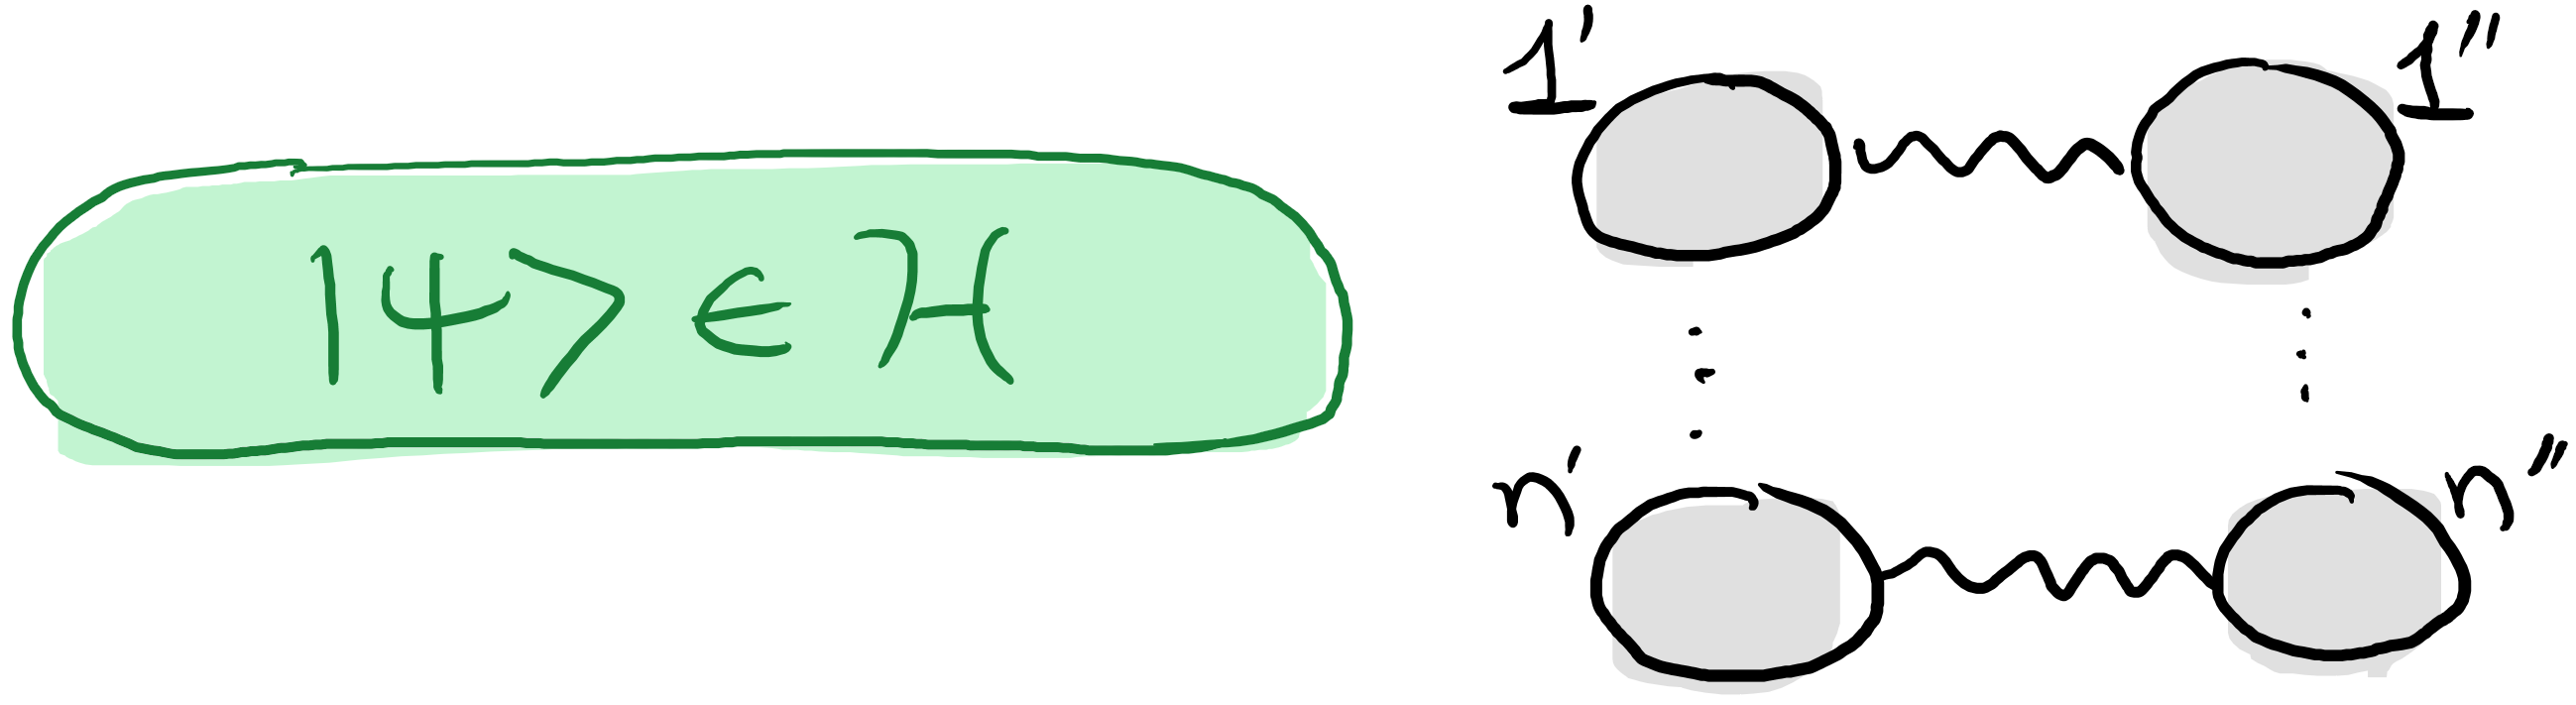
\includegraphics[scale=.07]{images/psiwitheprstates.png}
\caption{The state $\ket{\Psi_0}$ is given by $\ket \psi \otimes \ket{\EPRstate}^{\otimes n}$, where the EPR states are on qubits $1'$ and $1''$, $2'$ and $2''$, and so on.  To get $\ket \Psi$, swap qubit~$j'$ with the qubit in~$\H$ defined by $X_j, Z_j$, for $j = 1, \ldots, n$.  Observe that starting from $\ket \psi$ and depolarizing the $X_j, Z_j$ qubits, for $j = 1, \ldots, n$, is equivalent to tracing out all $j'$ and~$j''$ qubits from $\ketbra \Psi \Psi$.} \label{f:addneprstates}
\end{figure}

\begin{proof}[Proof of \thmref{t:statedependentnqubitprotocol}]
To analyze the protocol, we relate it to a separate protocol that is based on swapping qubits with halves of EPR states.  Observe that measuring either $X_i$ then $Z_i$, or $Z_i$ then $X_i$, and discarding the second measurement result, is equivalent to depolarizing the qubit.  Depolarizing a qubit is equivalent to swapping it with one half of $\ket{\EPRstate}$ and tracing out the original EPR state's registers.  Therefore, the protocol of \figref{f:statedependentnqubitprotocol} accepts with the same probability as the following protocol: 
\begin{enumerate}
\item Append to the system $n$ EPR states, on qubits labeled $1', 1'', \ldots, n', n''$.  Thus the system is in the state $\ket{\Psi_0} = \ket \psi \otimes \ket{\EPRstate}^{\otimes n} \in \H \otimes (\C^2_{1'} \otimes \C^2_{1''}) \otimes \cdots \otimes (\C^2_{n'} \otimes \C^2_{n''})$; see \figref{f:addneprstates}.  
\item For $i$ from $1$ up to $n$, swap the qubit defined by $X_i, Z_i$ with the new qubit~$i'$.  
\item Pick a uniformly random index~$j \in [n]$.  With equal probabilities $1/2$, measure either $X_j$ and~$\sigma^x_{j''}$, or $Z_j$ and $\sigma^z_{j''}$.  Accept if the measurement results are the same, both $+1$ or both~$-1$.  
\end{enumerate}
Indeed, for $\alpha \in \{x, z\}$, measuring $\sigma^\alpha_{j''}$ at the end of the protocol is equivalent to measuring $\sigma^\alpha_{j'}$ at the start, which is also equivalent to measuring just after swapping with the $X_j, Z_j$ qubit.  

If the protocol accepts with probability $1 - \epsilon$, then for probabilities $\epsilon_j$ satisfying $\epsilon = \tfrac{1}{n} \sum_j \epsilon_j$, we have $\min\!\big\{ \norm{\tfrac12 (\identity + X_j \otimes \sigma^x_{j''}) \ket \Psi}{}^2, \norm{\tfrac12 (\identity + Z_j \otimes \sigma^z_{j''}) \ket \Psi}{}^2 \big\} \geq 1 - 2  \epsilon_j$, where $\ket \Psi$ is the state after the swap gates in step~(2).  In particular, 
\begin{equation*}
\max\Big\{ \bignorm{X_j \otimes \sigma^x_{j''} \ket \Psi - \ket \Psi}, \bignorm{Z_j \otimes \sigma^z_{j''} \ket \Psi - \ket \Psi} \Big\} \leq 2 \sqrt{2 \epsilon_j}
 \enspace .
\end{equation*}
This implies that for any one-qubit operator $U_j$ acting on the $X_j, Z_j$ qubit, $U_j \ket \Psi \approx U_{j''}^T \ket \Psi$, where $U_{j''}$ is the same operator, but acting on the $j''$ qubit.  More precisely, if $U_j = \alpha_j \identity + \beta_j X_j + \gamma_j Z_j + \delta_j (i X_j Z_j)$ for complex scalars $\alpha_j, \beta_j, \gamma_j, \delta_j$, then $U_{j''}^T = \alpha_j \identity + \beta_j \sigma^x_{j''} + \gamma_j \sigma^z_{j''} - \delta_j \sigma^y_{j''}$; and, since $\max\{ \abs{\alpha_j}, \abs{\beta_j}, \abs{\gamma_j}, \abs{\delta_j} \} \leq \norm{U_j}$, 
\begin{align*}
\bignorm{(U_j - U_{j''}^T) \ket \Psi} 
&\leq (\abs{\beta_j} + \abs{\gamma_j} + 2 \abs{\delta_j}) \cdot 2 \sqrt{2 \epsilon_j} \\
&\leq 4 \norm{U_j} \cdot 2 \sqrt{2  \epsilon_j}
 \enspace .
\end{align*}
For each~$i$, let $\S_i$ be the operator on that swaps the $X_i, Z_i$ qubit with the new qubit~$i'$: $\S_i = \frac12 \big( \identity + X_i \otimes \sigma^x_{i'} + Z_i \otimes \sigma^z_{i'} + i (X_i Z_i) \otimes \sigma^y_{i'} \big)$.  
For $i \leq j$, let $\S_{i,j} = \S_i \S_{i+1} \ldots \S_j$ and $\S_{j,i} = \S_j \S_{j-1} \ldots \S_i$.  Thus $\ket \Psi = \S_{n,1} \ket{\Psi_0}$.  

Let $\hat P_i = \S_{n,i+1} P_i \S_{i+1,n} = \S_{n,i} \sigma^P_{i'} \S_{i,n} = \S_{n,1} \sigma^P_{i'} \S_{1,n}$.  As $[\sigma^P_{i'}, \sigma^Q_{j'}] = 0$ for $i \neq j$ and $P, Q \in \{X, Z\}$, so too $[\hat P_i, \hat Q_j] = 0$.  

Observe that 
\begin{equation} \label{e:switch1}
\hat U_j \ket \Psi = U_{j''}^T \ket \Psi
 \enspace ,
\end{equation}
 since 
\begin{align*}
\hat U_j \S_{n,1} \ket{\Psi_0} 
&= (\S_{n,1} U_{j'} \S_{1,n}) \S_{n,1} \ket{\Psi_0} \\
&= \S_{n,1} U_{j'} \ket{\Psi_0} \\
&= \S_{n,1} U_{j''}^T \ket{\Psi_0}
 \enspace ,
\end{align*}
where the last equality is because $\ket{\Psi_0}$ includes an EPR state between qubits $j'$ and~$j''$.  It follows that for any unitary $U$ acting only on the $X_j, Z_j$ qubit,
\begin{equation} \label{e:normbound0}
\bignorm{(U_j - \hat U_j) \ket \Psi} \leq 8 \sqrt{2 \epsilon_j}
 \enspace .
\end{equation}
Now consider a sequence of operators $U_{j_1}, \ldots, U_{j_k}$, where $U_j$ acts on the $X_j, Z_j$ qubit and $\norm{U_j} \leq 1$.  Then iterating $\hat U_j \ket \Psi = U_{j''}^T \ket \Psi$ gives 
\begin{align*}
\hat U_{j_1} \cdots \hat U_{j_k} \ket \Psi 
&= \hat U_{j_1} \cdots \hat U_{j_{k-1}} U_{j_k''}^T \ket \Psi \\
&= U_{j_k''}^T \hat U_{j_1} \cdots \hat U_{j_{k-1}} \ket \Psi \\
&= \cdots \\
&= U_{j_k''}^T \cdots U_{j_1''}^T \ket \Psi 
 \enspace .
\intertext{To continue, iterate on $U_j \ket \Psi \approx U_{j''}^T \ket \Psi$: }
&\approx U_{j_1} U_{j_k''}^T \cdots U_{j_2''}^T \ket \Psi \\
&\approx \cdots \\
&\approx U_{j_1} \cdots U_{j_k} \ket \Psi
 \enspace .
\end{align*}
The overall error satisfies 
\begin{equation*}
\bignorm{ U_{j_1} \cdots U_{j_k} \ket \Psi - \hat U_{j_1} \cdots \hat U_{j_k} \ket \Psi } 
\leq k \cdot 4 \max \norm{U_{j_\ell}} \cdot 2 \sqrt{2 \epsilon_{j_\ell}}
= O(k \sqrt{n \epsilon})
 \enspace .  \qedhere
\end{equation*}
\end{proof}

In \thmref{t:statedependentnqubitprotocol}, the definition of $\ket \Psi$ requires adding to $\H$ an additional ancilla register $(\C^2)^{\otimes 2n}$.  It is therefore not clear that the theorem should imply an exponential lower bound on the dimension of~$\H$.  In fact, though, it does lower-bound $\dim \H$: 

\begin{corollary} \label{t:statedependentnqubitdimensionlowerbound}
If the protocol in \figref{f:statedependentnqubitprotocol} accepts with probability at least $1 - \epsilon$, then 
\begin{equation*}
\dim \H \geq \big( 1 - O(n^2 \epsilon) \big) \, 2^n
 \enspace .
\end{equation*}
\end{corollary}

\begin{proof}
For $(a, b) \in \{0,1\}^n \times \{0,1\}^n$ let 
\begin{equation*}
\ket{\Psi_{a,b}} 
= \big( X_n^{a_n} Z_n^{b_n} \big) \cdots \big( X_1^{a_1} Z_1^{b_1} \big) \ket \Psi
 \enspace .
\end{equation*}

\begin{claim}
The $\ket{\Psi_{a,b}}$ satisfy 
$\dim \Span \{ \ket{\Psi_{a,b}} \} \geq \big( 1 - O(n^2 \epsilon) \big) 4^n$.  
\end{claim}

\begin{proof}
Let $B = \sum_{a, b} \ketbra{\Psi_{a,b}}{a, b}$.  
Adopt the notation from the proof of \thmref{t:statedependentnqubitprotocol}.  
For $k \in \{0, \ldots, n\}$ define $\ket{\hat \Psi^{(k)}_{a,b}}$ similarly to $\ket{\Psi_{a,b}}$, except using the operators $\hat X_j$ and $\hat Z_j$ in place of $X_j$ and~$Z_j$ for $j \leq k$. Thus $\ket{\hat \Psi^{(0)}_{a,b}} = \ket{ \Psi_{a,b}}$.  Let $\ket{\hat \Psi_{a,b}} = \ket{ \hat \Psi^{(n)}_{a,b}}$ and define $\hat{B}$ as $B$ using the $\ket{\hat \Psi_{a,b}}$ instead of $\ket{\Psi_{a,b}}$.  Using the triangle inequality and $\norm{X_j}, \norm{Z_j} \leq 1$,
\begin{align}
\bignorm{ \ket{\hat \Psi_{a,b}} - \ket{\Psi_{a,b}} } 
&\leq \sum_{k=1}^n \bignorm{\ket{\hat \Psi^{(k)}_{a,b}} - \ket{\hat \Psi^{(k-1)}_{a,b}}} \notag\\
&\leq \sum_{k=1}^n \Bignorm{\big( \hat X_k^{a_k} \hat Z_k^{b_k} - X_k^{a_k} Z_k^{b_k} \big) \Big( \prod_{j < k} \hat X_j^{a_j} \hat Z_j^{b_j} \Big) \ket{\Psi}}
 \enspace . \label{e:normbound2a}
\end{align}
By Eq.~\eqnref{e:switch1} from the proof of \thmref{t:statedependentnqubitprotocol}, $\hat P_j \ket \Psi = P_{j''}^T \ket \Psi$, where $P_{j''}$ acts only on the $j''$ ancilla qubit and therefore commutes with all $Q_k$ and $\hat Q_k$.  Thus for any~$k \in [n]$, 
\begin{align*}
\big( \hat X_k^{a_k} \hat Z_k^{b_k} - X_k^{a_k} Z_k^{b_k} \big) \Big( \prod_{j < k} \hat X_j^{a_j} \hat Z_j^{b_j} \Big)\ket \Psi
&=\Big( \prod_{j < k} \big(X_{j''}^{a_j} Z_{j''}^{b_j} \big)^T \Big) \big(\hat X_k^{a_k} \hat Z_k^{b_k} - X_k^{a_k} Z_k^{b_k} \big) \ket \Psi
 \enspace .
\end{align*}
Thus starting from Eq.~\eqnref{e:normbound2a} and applying~\eqnref{e:normbound0}, we obtain the bound
\begin{equation} \label{e:normbound2}
\bignorm{ \ket{\hat \Psi_{a,b}} - \ket{\Psi_{a,b}}} 
\leq \sum_{k=1}^n 8 \sqrt{2 \epsilon_k}
  \enspace .
\end{equation}
Moreover, the $\ket{\hat \Psi_{a,b}}$ vectors are orthonormal: 
\begin{align*}
\braket{\hat \Psi_{a,b}}{\hat \Psi_{c,d}}
&= \bra{\Psi_0} \S_{1,n} \prod_{j=1}^n \big( \hat Z_j^{b_j} \hat X_j^{a_j + c_j} \hat Z_j^{d_j} \big) \S_{n,1} \ket{\Psi_0} \\
&= (-1)^{(a + c) \cdot b} \bra{\EPRstate}^{\otimes n} \prod_{j=1}^n \big( (\sigma^x_{j'})^{a_j+c_j} (\sigma^z_{j'})^{b_j+d_j} \big) \ket{\EPRstate}^{\otimes n} \\
&= \delta_{a,c} \delta_{b,d}
 \enspace .
\end{align*}
Therefore $\hat B$ is an isometry.  Its singular values are $1$ with multiplicity $4^n$.  Let $\lambda_1 \geq \cdots \geq \lambda_{4^n} \geq 0$ be the singular values of~$B$.  (Some $\lambda_i$ may be zero.)  Then, relating the singular values of $B$ and~$\hat B$ to the Frobenius norm of their difference, 
\begin{align*}
\sum_i \abs{\lambda_i - 1}^2 
&\leq \norm{B - \hat B}{}_F^2 \\
&= \sum_{a,b} \bignorm{\ket{\Psi_{a,b}} - \ket{\hat \Psi_{a,b}}}^2 \\
&\leq 4^n \cdot 128 \cdot n^2 \epsilon
 \enspace ,
\end{align*}
where the last bound is by Eq.~\eqnref{e:normbound2} and $\sum_k \epsilon_k = n \epsilon$.  Since the left-hand side is at least $4^n - \rank(B)$, we obtain $\rank(B) \geq \big( 1 - O(n^2 \epsilon) \big) 4^n$.  
\end{proof}

Let $\ket \Psi$ have Schmidt decomposition $\ket \Psi = \sum_{i = 1}^{d} \sqrt{p_i} \ket{u_i} \otimes \ket{v_i}$ across the partition $\H$, $(\C^2)^{\otimes 2 n}$.  Extend the set $\{\ket{u_1}, \ldots, \ket{u_d}\}$, if necessary, to form an orthonormal basis for~$\H$.  The vectors $\ket{\Psi_{a,b}}$ are obtained from $\ket \Psi$ by applying operators $X_j, Z_j$ supported only on~$\H$.  Therefore, they lie in the span of $\{ \ket{u_i} \otimes \ket{v_j} : i \in [\dim \H], j \in [d] \}$.  In particular, $\dim \Span \{\ket{\Psi_{a,b}}\} \leq d \dim \H \leq (\dim \H)^2$, as desired.  
\end{proof}

\begin{remark}
In \thmref{t:manynearlyindependentqubits}, different qubits overlapping by $\epsilon = O(1/n)$ already implies $\dim \H \geq 2^n$.  In contrast, in \corref{t:statedependentnqubitdimensionlowerbound}, $\epsilon$ must be exponentially small before $\dim \H \geq 2^n$ is required.  Is this polynomial versus exponential separation a consequence of loose analysis, an inherent drawback of the protocol in \figref{f:statedependentnqubitprotocol}, or an inherent property of any efficient state-dependent qubit testing protocol?  

\newcommand\restrict[1]{\raisebox{-.5ex}{$|$}{}_{#1}^{}}

The following example suggests at least that our analysis is not too loose.   Let $\H = \Span\{ \ket x : x \neq 0^n, 1^n \} \subset (\C^2)^{\otimes n}$.  Define $n$ qubits by $Z_j = \sigma^z_j \restrict{\H}$ and $X_j = \sigma^x_j \restrict{\H} + \sigma^x_j (\ketbra{1^n}{0^n} + \ketbra{0^n}{1^n}) \sigma^x_j$.  That is, while $\sigma^x_j$ maps the basis states $\sigma^x_j \ket{0^n}$ and $\sigma^x_j \ket{1^n}$ outside of~$\H$, $X_j$ instead maps them to each other.  Even though $\dim \H = 2^n - 2 < 2^n$, it seems that these $n$ qubits can pass our testing protocol with probability $1 - 1/\exp(n)$.\footnote{A natural generalization of this construction removes all strings of Hamming weight $< t$ or $> n-t$, with $Z_j = \sigma^z_j \restrict{\H}$ and $X_j \ket x = \sigma^x_j \ket x$ except $X_j \ket x = \ket{\overline x}$ when $\sigma^x_j \ket x$ would cross the boundary. We omit the details.}  
\end{remark}


\ifx\compilefullpaper\undefined  
%\addcontentsline{toc}{section}{References}
\bibliographystyle{alpha-eprint}
\bibliography{q}

\end{document}
\fi